\documentclass[article,11pt]{mwrep}
\usepackage[a4paper, margin=2.5cm]{geometry}
\usepackage[utf8]{inputenc}
\usepackage[T1]{fontenc}
\usepackage{polski}
\usepackage{graphicx}
\usepackage{xcolor}
\usepackage{hyperref}
\usepackage{amsmath}
\usepackage{amsthm}
\usepackage{amssymb}
\usepackage{bm}
\usepackage{enumitem}
\usepackage{mathrsfs}
\usepackage{tikz}
\usepackage{float}


\newcommand{\R}{{\mathbb R}}
\newcommand{\Z}{{\mathbb Z}}
\newcommand{\N}{{\mathbb N}}
\newcommand{\Q}{{\mathbb Q}}
\newcommand{\C}{{\mathbb C}}
\newcommand{\M}{{\textnormal{M}}}

\title{Dokumentacja aplikacji}
\author{Kamil Jarkowski, Damian Forma, Paweł Drzyzga}
\date{\today}

\begin{document}

\maketitle

\chapter{Wprowadzenie}

Aplikacja ta jest narzędziem służącym do:
\begin{itemize}
    \item Obliczania średnicy zbiorów,
    \item Obliczania odległości między zbiorami,
    \item (eksperymentalnie) Rysowania kul otwartych, domkniętych, jak i sfer w przestrzeni dwuwymiarowej.
\end{itemize}


Sama aplikacja została udostepniona przy pomocy oficjalnej strony streamlit pod linkiem \url{https://kursapp-pg9qzqkjjdkuyezpwiurdn.streamlit.app/}. Cały kod źródłowy aplikacji jest dostępny na platformie GitHub pod adresem \url{https://github.com/Qertal/KursStreamlit/tree/main/projekt_topo}.

W całości została ona wykonana w języku Python, głównie przy użyciu biblioteki \textbf{Numpy} do obliczeń numerycznych oraz \textbf{Streamlit} do stworzenia interfejsu użytkownika. Aplikacja jest prosta w obsłudze, a jej działanie jest intuicyjne. W tej dokumentacji zostaną przedstawione poszczególne sekcje aplikacji oraz ich funkcjonalności.

\chapter{Pierwsze wejście na stronę aplikacji}

Możliwe, że pierwsze wejście na stronę aplikacji będzie trwało dłużej niż zwykle. Jest to spowodowane tym, że aplikacja jest uruchamiana na serwerze, a nie lokalnie. Dodatkowo, możliwe, że aplikacja będzie w stanie uśpienia (\ref{rys:usp}). Wtedy wystarczy kliknąć przycisk z napisem \textbf{Yes, get this app back up!}, a aplikacja zostanie uruchomiona ponownie.

%\includegraphics[]{Obraz1.png}

\begin{figure}[H] 
    \centering
    \includegraphics[width=0.8\textwidth]{figure/Obraz1.png}
    \caption{Uśpiona aplikacja}\label{rys:usp}
\end{figure}

\section{Strona główna aplikacji}

Na stronie głównej aplikacji (\ref{rys:sg}) znajdują się wypisani autorzy, a także po lewej stronie mały panel nawigacyjny, który pozwala na przejście do poszczególnych sekcji aplikacji, poprzez kliknięcie w odpowiednią część. Warto zwrócić uwagę, że w każdej chwili można wrócić do strony głównej klikając przycisk \textbf{Strona Główna}. 

\begin{figure}[H] 
    \centering
    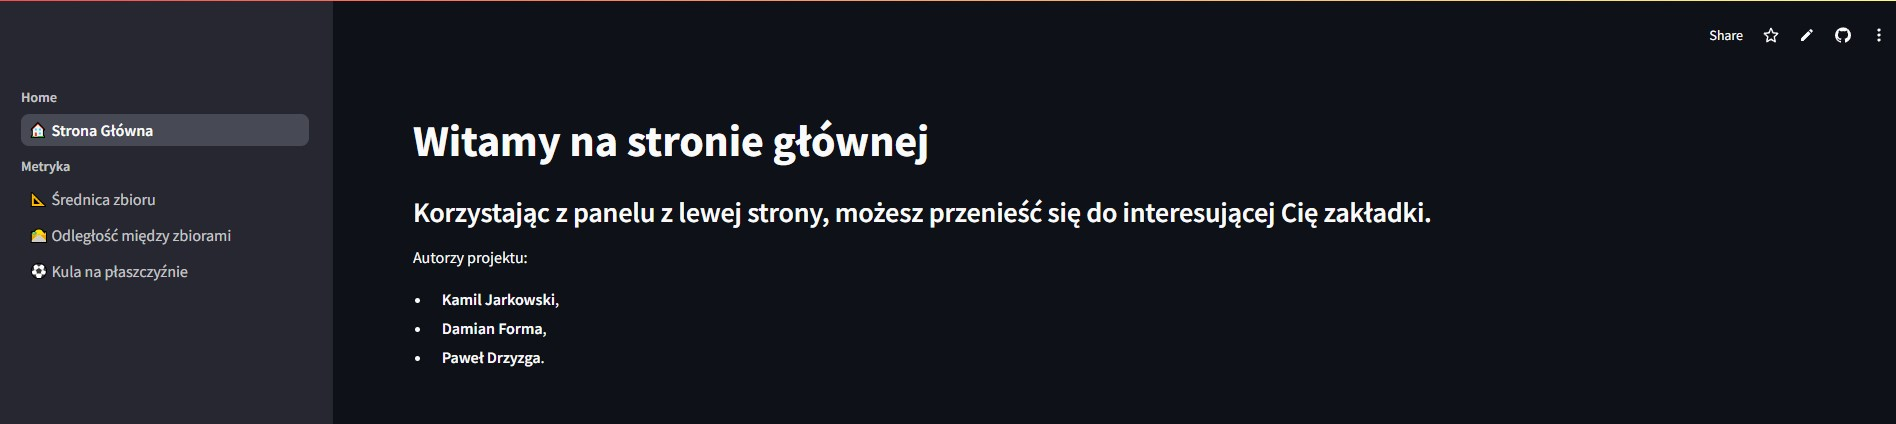
\includegraphics[width=0.8\textwidth]{figure/Screenshot_1.jpg}
    \caption{Strona Główna}\label{rys:sg}
\end{figure}

Przejdźmy do pierwszej sekcji, a mianowicie do \textbf{Średnica zbioru}.

\chapter{Średnica zbioru}

Klikając w przycisk \textbf{Średnica zbioru} w polu nawigacji, przenosi nas na stronę (\ref{rys:sz}), gdzie możemy skorzystać z kalkulatora średnicy zbioru. 

\begin{figure}[H] 
    \centering
    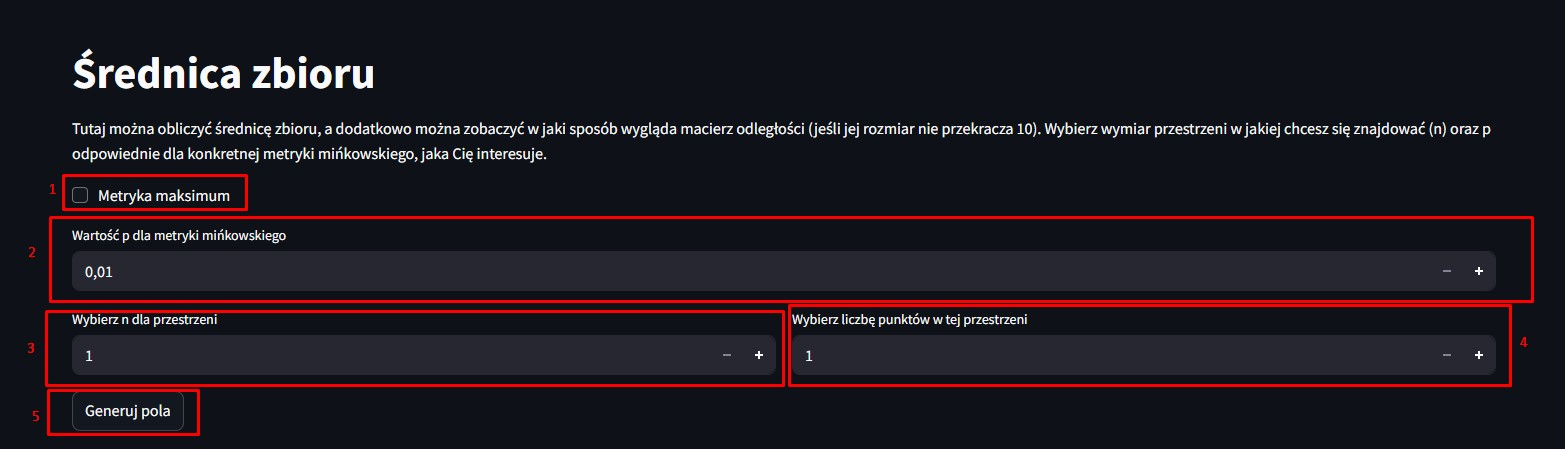
\includegraphics[width=0.8\textwidth]{figure/Screenshot_2.jpg}
    \caption{Formularz \textbf{Średnica zbioru}}\label{rys:sz}
\end{figure}

Możemy zauważyć, różne sposoby interakcji ze stroną (numerki z listy poniżej są zgodne z numerkami na rysunku):
\begin{enumerate}
    \item W tym miejscu, możemy wybrać, czy metryka z której chcemy skorzystać, jest to metryka Czebyszewa, z racji na jej utrudnioną w sposobie zapisu symbolikę, została ona odizolowana od reszty, od klasycznego wyboru rodzaju metryki.
    \item Jeśli nie zdecydujemy się na wybór metryki Czebyszewa, możemy określić jakie użyjemy p ($p\in\R_+$) dla metryki Minkowskiego, czyli $d(x,y)=\left(\sum_{i=1}^n |x_i-y_i|^p\right)^{1/p}$. Możliwe jest wybranie wartości $p < 1$, co skutkuje użyciem wzoru $d(x,y)=\left(\sum_{i=1}^n |x_i-y_i|^p\right)$. W momencie gdy wybierzemy metrykę Czebyszewa, pole to automatycznie znika.
    \item W tym miejscu wybieramy wymiary przestrzeni, w której będziemy pracować. Czyli chodzi konkretnie o $n$ dla przestrzeni $\R^n$ ($n\in\N\backslash \{0\} $).
    \item Tutaj wybieramy ile punktów będzie w naszej przestrzeni. Wybierając $>10$ punktów, na sam koniec, nie zostanie wyświetlona macierz odległości, z racji na jej rozmiar. Warto mieć to na uwadzę.
    \item Na koniec mamy przycisk \textbf{Generuj pola}, który generuje pola, które są potrzebne do wpisania punktów.
\end{enumerate}

Po kliknięciu przycisku \textbf{Generuj pola}, zostanie wyświetlona "siatka pól" (\ref{rys:sp}), gdzie możemy wpisać współrzędne punktów, które chcemy użyć do obliczenia średnicy zbioru. Warto zauważyć, że pola są automatycznie uzupełnione losowymi liczbami całkowitymi z przedziału $[-15,15]$, ale można je edytować. Po wprowadzeniu punktów, należy kliknąć przycisk \textbf{Oblicz}.

\begin{figure}[H] 
    \centering
    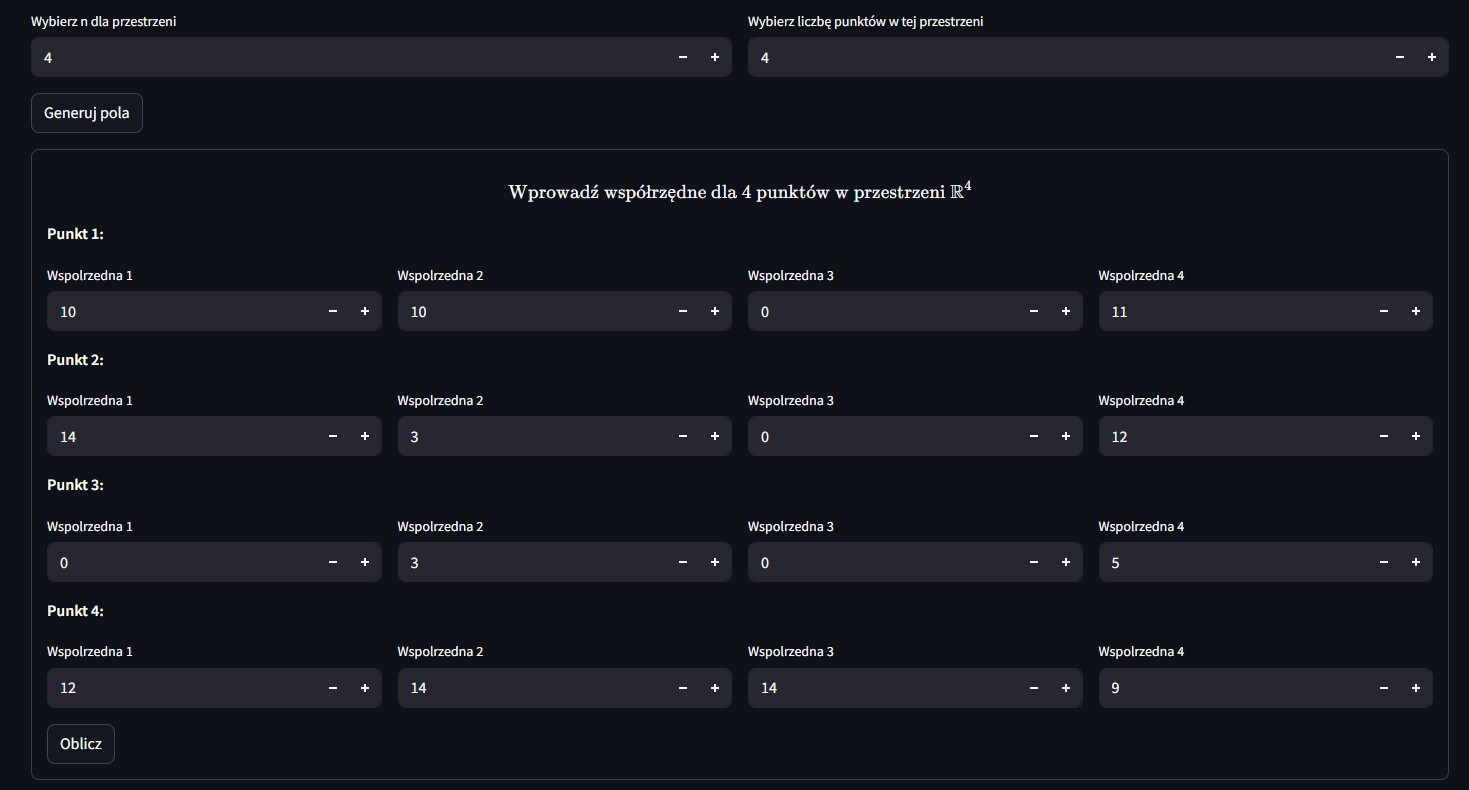
\includegraphics[width=0.8\textwidth]{figure/Screenshot_3.jpg}
    \caption{Formularz \textbf{Średnica zbioru 2}}\label{rys:sp}
\end{figure}

Po kliknięciu przycisku \textbf{Oblicz}, pierwsze co zostanie wyświetlone, to macierz odległości między punktami (\ref{rys:mo}). Jest to macierz symetryczna, gdzie $d_{ij}$ to odległość między punktem $i$ a punktem $j$. Następnie zostanie wyświetlona średnica zbioru, czyli maksymalna odległość między punktami.

\begin{figure}[H] 
    \centering
    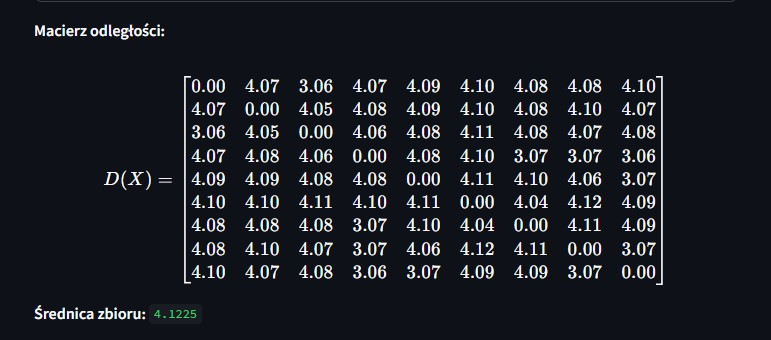
\includegraphics[width=0.8\textwidth]{figure/Screenshot_4.jpg}
    \caption{Macierz odległości i średnica zbioru}\label{rys:mo}
\end{figure}

\chapter{Odległość między zbiorami}

Teraz z lewegu panelu wybieramy przycisk \textbf{Odległość między zbiorami}, co przenosi nas do sekcji poświęconej (jak sama nazwa wskazuje) obliczaniu odległości między dwoma zbiorami (\ref{rys:omz}). 

\begin{figure}[H] 
    \centering
    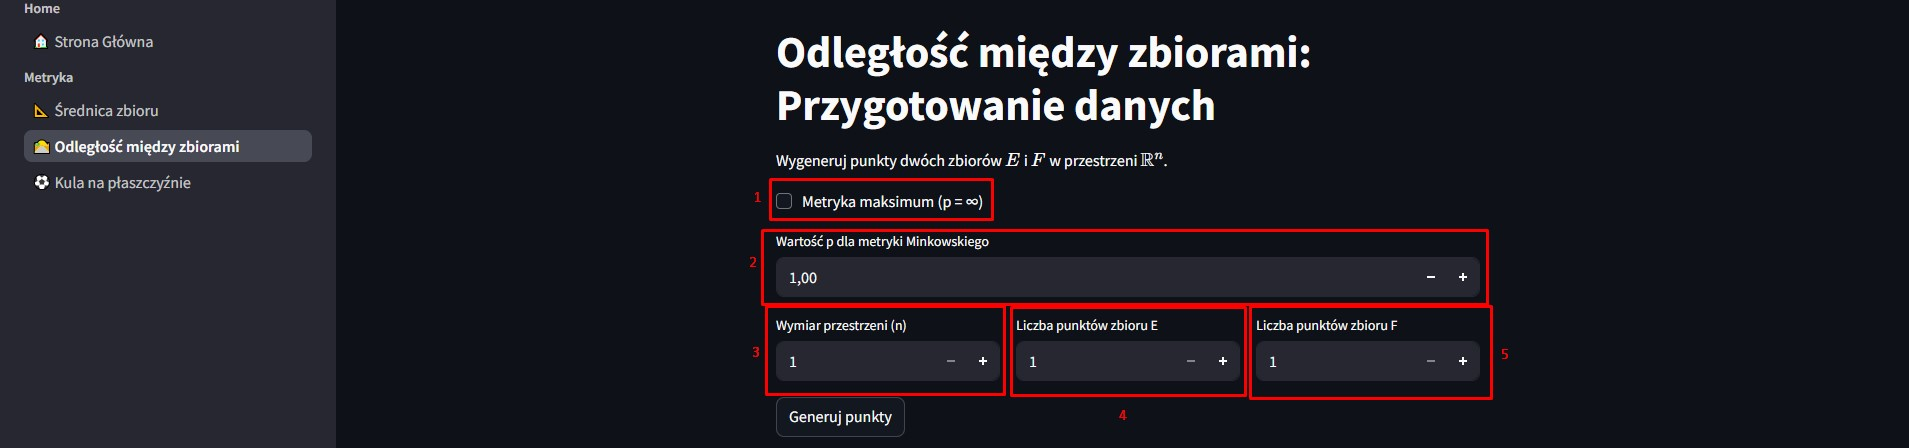
\includegraphics[width=0.8\textwidth]{figure/Screenshot_5.jpg}
    \caption{Odległość między zbiorami}\label{rys:omz}
\end{figure}

Tak jak wcześniej, mamy różne sposoby interakcji ze stroną (numerki z listy poniżej są zgodne z numerkami na rysunku):

\begin{enumerate}
    \item Tak jak wcześniej, możemy wybrać metrykę Czebyszewa, która jest odizolowana od reszty, ze względu na jej utrudnioną w sposobie zapisu symbolikę.
    \item W momencie, kiedy nie zdecydujemy się na metrykę Czebyszewa, możemy wybrać wartość $p$ dla metryki Minkowskiego, tak jak wcześniej.
    \item W tym miejscu wybieramy wymiary przestrzeni, w której będziemy pracować. Czyli chodzi konkretnie o $n$ dla przestrzeni $\R^n$ ($n\in\N\backslash \{0\} $).
    \item Tutaj wybieramy ile punktów będzie w pierwszym zbiorze E.
    \item Tutaj wybieramy ile punktów będzie w drugim zbiorze F.
\end{enumerate}

Po kliknięciu przycisku \textbf{Generuj punkty}, zostaną wygenerowane pola, w które możemy wpisać współrzędne punktów zbiorów $E$ i $F$ (\ref{rys:op}). Warto zauważyć, że pola są automatycznie uzupełnione losowymi liczbami całkowitymi z przedziału $[-15,15]$, ale można je edytować. Po wprowadzeniu punktów, należy kliknąć przycisk \textbf{Oblicz}. Wszystko to jest analogiczne do poprzedniej sekcji, z tą różnicą, że mamy dwa zbiory punktów.

\begin{figure}[H] 
    \centering
    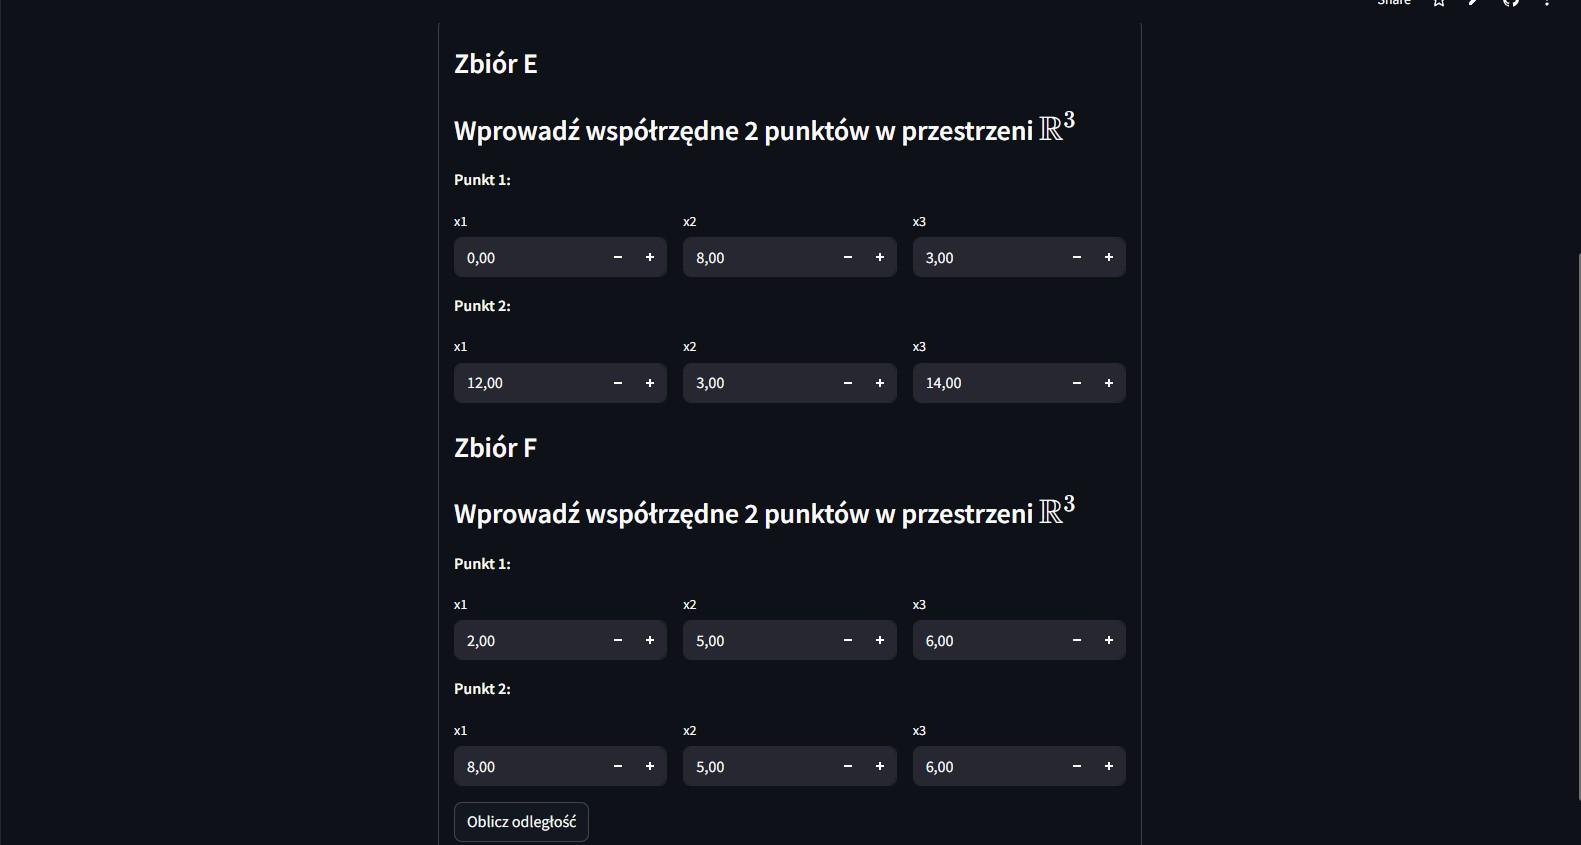
\includegraphics[width=0.8\textwidth]{figure/Screenshot_6.jpg}
    \caption{Odległość między zbiorami: pola}\label{rys:op}
\end{figure}

Po zdefiniowaniu punktów, klikamy przycisk \textbf{Oblicz odległość}, a aplikacja wypisze najpierw punkty dla obu zbiorów, a następnie obliczy odległość między zbiorami (\ref{rys:ow}).

\begin{figure}[H] 
    \centering
    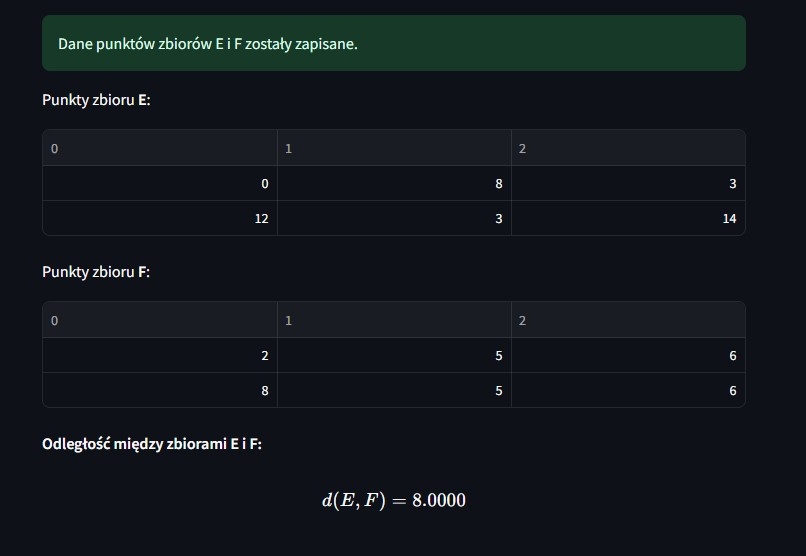
\includegraphics[width=0.8\textwidth]{figure/Screenshot_7.jpg}
    \caption{Odległość między zbiorami: wyniki}\label{rys:ow}
\end{figure}

\chapter{Rysowanie kul i sfer (eksperymentalnie)}

W tej sekcji aplikacji możemy rysować kule otwarte, domknięte oraz sfery w przestrzeni dwuwymiarowej. Aby skorzystać z tej funkcji, należy kliknąć przycisk \textbf{Kule na płaszczyźnie} (tak, jestem świadomy tego, ze sfera nie jest kulą), co przeniesie nas do sekcji (\ref{rys:rk}). 

\begin{figure}[H] 
    \centering
    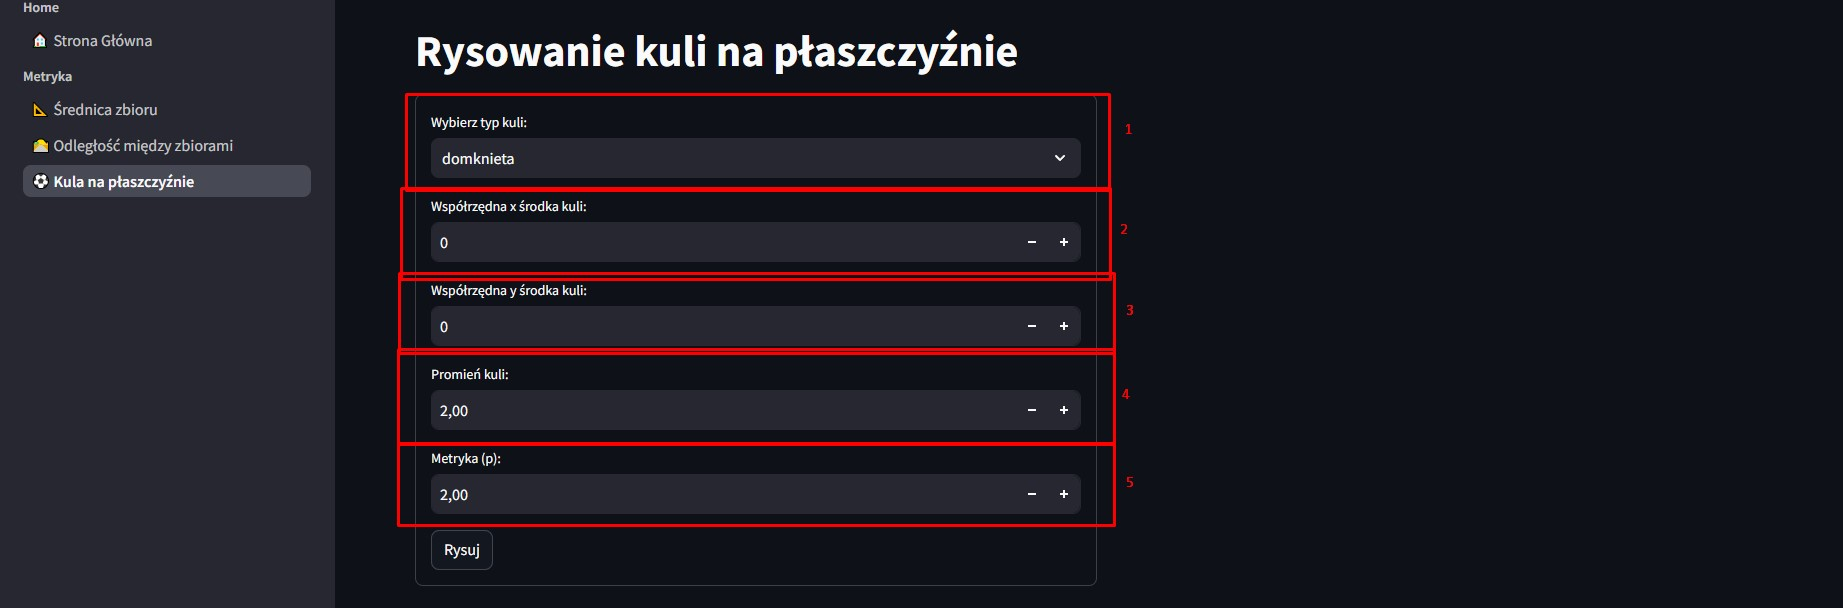
\includegraphics[width=0.8\textwidth]{figure/Screenshot_8.jpg}
    \caption{Rysowanie kul i sfer}\label{rys:rk}
\end{figure}

W tej sekcji mamy możliwość wyboru:
\begin{enumerate}
    \item Wybieramy czy chcemy rysować kulę otwartą, domkniętą czy sferę (chociaż \textbf{Wybierz typ kuli} może być mylące, to tak, da się wybrać sferę).
    \item Wybieramy pierwszą współrzędną środka kuli/sfery.
    \item Wybieramy drugą współrzędną środka kuli/sfery.
    \item Wybieramy promień kuli/sfery. 
    \item Wybieramy metrykę. Nie ma tutaj niestety do wyboru metryki Czebyszewa. Jednak z punktu widzenia stricte rysowania, możemy wybrać górną granicę $p$ jaka jest narzucona, w tym przypadku jest to $p=75$. Wartość ta bardzo dobrze przybliża kule bądź sferę w przestrzeni dwuwymiarowej z metryką Czebyszewa. 
\end{enumerate}

Warto wspomnieć, ze zostało wprowadzone tutaj troche limitów, są one skutkiem ograniczeń przy rysowaniu wykresów i generowaniu punktów, zarówno ze strony logicznej jak i technicznej (ograniczenia złożoności obliczeniowej). Głównie chodzi o to że:
\begin{enumerate}
    \item promień kuli/sfery musi być z przedziału $[1.5, 10]$ (sam promień paradoksalnie nie ma zbyt dużego wpływu na to jak my ten rysunek i tak będziemy widzieć),
    \item p dla metryki Minkowskiego musi być z przedziału $[0.2, 75]$ 
\end{enumerate}

Klikając przycisk \textbf{Rysuj}, aplikacja wygeneruje wykres z kulą/sferą w przestrzeni dwuwymiarowej (\ref{rys:rw}). 

\begin{figure}[H] 
    \centering
    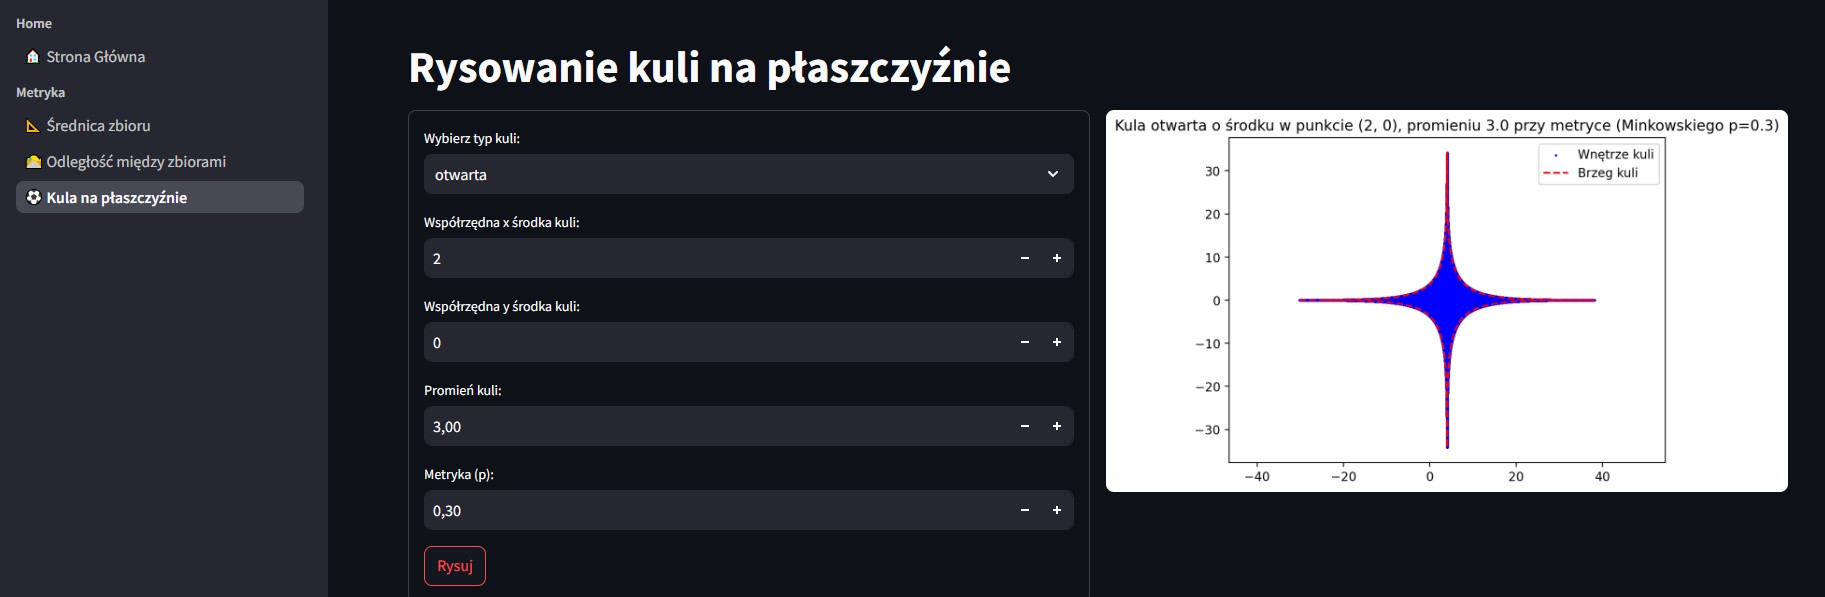
\includegraphics[width=0.8\textwidth]{figure/Screenshot_9.jpg}
    \caption{Rysowanie kul i sfer: wykres}\label{rys:rw}
\end{figure}

\chapter{Podsumowanie i możliwości rozwoju}

Jak widać, aplikacja jest dośc prosta w budowie jak i w obsłudze. Spełnia jednak ona swoje zadanie, czyli pozwala na obliczanie średnicy zbiorów, odległości między zbiorami oraz (poza koncertowo) rysowanie kul otwartych, domkniętych i sfer w przestrzeni dwuwymiarowej. W ramach rozwoju aplikacji, można by pomyśleć o obsłudzie wyrażeń niewymiernych przy obliczaniu średnicy zbiorów, czy też odległości między zbiorami. Dodatkowo można by dodać możliwość wyboru pomiędzy obliczeniami numerycznymi a symbolicznymi, co pozwoliłoby na uzyskanie dokładniejszych wyników. Może to być przydatne narzędzie dla studentów matematyki, którzy są na początku swojej drogi z topologią.

\end{document}
